\documentclass[conference]{IEEEtran}
\IEEEoverridecommandlockouts

\usepackage[T1]{fontenc}
\usepackage[utf8]{inputenc}
\usepackage[brazilian]{babel}
\usepackage{cite}
\usepackage{amsmath,amssymb,amsfonts}
\usepackage{graphicx}
\usepackage{booktabs}
\usepackage{xcolor}
\usepackage[hyphens]{url}
\def\BibTeX{{\rm B\kern-.05em{\sc i\kern-.025em b}\kern-.08em
    T\kern-.1667em\lower.7ex\hbox{E}\kern-.125emX}}
\begin{document}

\title{Comparação de modelos de aprendizado de máquina para estimativa do ganho médio diário de bovinos de corte}

\author{\IEEEauthorblockN{Euler Gomes da Rocha}
\IEEEauthorblockA{\textit{Departamento de Engenharia e Computação} \\
\textit{Instituto Federal de Minas Gerais -- Campus Bambuí}\\
Bambuí, Brasil \\
eulergomesrocha@gmail.com
}
\and
\IEEEauthorblockN{Ciniro Aparecido Leite Nametala}
\IEEEauthorblockA{\textit{Departamento de Engenharia e Computação} \\
\textit{Instituto Federal de Minas Gerais -- Campus Bambuí}\\
Bambuí, Brasil \\
ciniro.nametala@ifmg.edu.br
}
\and
\IEEEauthorblockN{Tamires Martins Rezende}
\IEEEauthorblockA{\textit{Fundação para Inovações Tecnológicas - FITec Labs} \\
Belo Horizonte, Brasil \\
inctamires@gmail.com
}
}

\maketitle

\begin{abstract}
O ganho médio diário de peso (GMD) orienta decisões de manejo e suplementação na pecuária de corte. Este trabalho compara regressão linear, XGBoost, uma rede neural densa (MLP) e o TabPFN, um modelo de fundação para dados tabulares, na estimativa do GMD de 245 bovinos de duas propriedades de Bambuí (MG), descritos por nove variáveis de animal, manejo, suplementação e clima, avaliando a generalização para lotes e propriedades não vistos no treinamento. A avaliação combinou validação cruzada estratificada por propriedade, validação cruzada agrupada por lote e treinamento em uma propriedade com teste na outra. Na validação por propriedade, o TabPFN ($R^2 = 0{,}86$; erro absoluto médio de 0,015~kg/dia) e a MLP ($R^2 = 0{,}82$; 0,028~kg/dia) superaram o XGBoost ($R^2 = 0{,}51$) e a regressão linear ($R^2 = 0{,}43$). Com validação agrupada por lote, o $R^2$ de todos os modelos diminuiu, e nenhum modelo generalizou de forma confiável para a outra propriedade.
\end{abstract}

\begin{IEEEkeywords}
aprendizado de máquina, bovinos de corte, ganho médio diário, TabPFN, análise exploratória, validação cruzada.
\end{IEEEkeywords}

\noindent\textbf{\textit{Abstract}---}Average daily gain (ADG) guides management and supplementation decisions in beef cattle production. We compare linear regression, XGBoost, a dense neural network (MLP) and TabPFN, a tabular foundation model, for estimating the ADG of 245 cattle from two farms in Bambuí, Brazil, described by nine animal, management, supplementation and climate variables, and evaluate generalization to unseen cohorts and farms. Models were assessed with farm-stratified cross-validation, cohort-grouped cross-validation, and training on one farm with testing on the other. Under farm-stratified cross-validation, TabPFN ($R^2 = 0.86$; mean absolute error 0.015~kg/day) and the MLP ($R^2 = 0.82$; 0.028~kg/day) outperformed XGBoost ($R^2 = 0.51$) and linear regression ($R^2 = 0.43$). Under cohort-grouped validation the $R^2$ of every model decreased, and no model generalized reliably to the other farm.

\section{Introdução}

O agronegócio brasileiro encerrou 2025 com exportações recordes de US\$~169 bilhões~\cite{ministerio2026}. Na fazenda, o ganho médio diário de peso (GMD) é o indicador que resume o desempenho de um animal ou lote~\cite{alencastrofilho2017}: é com ele que se projeta a data de abate, se avalia a resposta à suplementação em pastagens tropicais~\cite{tambara2021} e se decide o manejo nutricional. Prever o GMD com antecedência ou estimá-lo a partir de registros de rotina é, portanto, uma necessidade prática.

A aprendizagem de máquina é cada vez mais usada em sistemas agropecuários, com bovinos entre os animais mais estudados e redes neurais entre as técnicas mais eficientes~\cite{benos2021}, e a pecuária de precisão combina sensores e algoritmos para apoiar decisões de manejo~\cite{curti2023}. Para ganho e peso de bovinos de corte há trabalhos com regressão, árvores e boosting~\cite{tuyishime2025}, classificação com árvores, redes neurais e regressão logística~\cite{grzesiak2023} e predição genômica de características de crescimento~\cite{hay2024}.

Divisões aleatórias de animais medem o desempenho para animais semelhantes aos do treino, mas não para lotes ou propriedades novas, o que motiva avaliar também com lotes e propriedades inteiros fora do treino. Além disso, modelos de fundação para dados tabulares, como o TabPFN~\cite{hollmann2025tabpfn}, foram propostos para conjuntos de até 10 mil amostras, faixa em que se situa este estudo.

As contribuições deste trabalho são: (i)~a comparação de regressão linear, XGBoost~\cite{chen2016xgboost}, uma MLP e o TabPFN em um mesmo conjunto de 245 bovinos, com os mesmos particionamentos e métricas; (ii)~uma avaliação em três níveis de rigor (por animal e propriedade, por lote e entre propriedades); (iii)~a medição da queda de desempenho quando lotes inteiros são retirados do treino; e (iv)~a interpretação do melhor modelo com valores SHAP~\cite{lundberg2017shap}.

O restante do artigo está organizado assim: a Seção~\ref{sec:rel} resume trabalhos relacionados; a Seção~\ref{sec:met} descreve os dados, os modelos e a validação; a Seção~\ref{sec:res} apresenta os resultados; a Seção~\ref{sec:disc} os discute, com as limitações; e a Seção~\ref{sec:concl} conclui.

\section{Trabalhos relacionados}\label{sec:rel}

Revisões recentes mostram que o aprendizado de máquina na agricultura abrange manejo de culturas, água, solo e pecuária, com bovinos e ovinos entre os animais mais investigados~\cite{benos2021}, e que sensores e algoritmos têm sido combinados em produção e reprodução animal~\cite{curti2023}.

Sobre o ganho de peso, Tuyishime e Adewusi~\cite{tuyishime2025} compararam regressão linear, árvore de decisão, XGBoost e regressão por vetores de suporte para prever o peso aos 36 meses; a árvore de decisão teve o melhor desempenho ($R^2 = 0{,}927$; erro absoluto médio de 2,21~kg), os pesos em idades anteriores foram os preditores mais fortes e variáveis ambientais tiveram efeito moderado. Grzesiak et al.~\cite{grzesiak2023} compararam árvores de decisão, redes neurais e regressão logística para classificar o ganho diário de bezerros de corte das raças Simmental e Limousin, com a floresta aleatória apresentando a melhor área sob a curva (0,82 e 0,81). Hay~\cite{hay2024} comparou floresta aleatória, máquinas de vetores de suporte, redes convolucionais e perceptrons multicamadas com o GBLUP na predição genômica de peso ao nascer, à desmama e ao sobreano, e o GBLUP foi superior no conjunto, o que lembra que métodos estatísticos clássicos podem superar modelos de aprendizado de máquina.

Outra linha estima o peso a partir de imagens: imagens tridimensionais de vacas leiteiras~\cite{gebreyesus2023}, comparações de modalidades de dados com aprendizado profundo~\cite{afridi2024} e segmentação semântica combinada com redes de retropropagação~\cite{xu2024}. Esses trabalhos têm outro alvo (o peso em um instante, não o ganho em um ciclo) e outro tipo de entrada. Do lado zootécnico, a meta-análise de Tambara et al.~\cite{tambara2021} trata do efeito da suplementação sobre a produção de bovinos de corte em pastagens tropicais brasileiras nas águas e na seca, e motiva a inclusão de variáveis de suplementação e de estação.

Em relação a esses estudos, o presente trabalho usa dados observacionais de campo com ciclos longos (de 43 a 1253 dias), compara quatro famílias de modelos, incluindo um modelo de fundação tabular, e concentra a análise no desenho da validação.

\section{Materiais e métodos}\label{sec:met}

\subsection{Dados}

O conjunto contém 245 bovinos fêmeas de duas propriedades da região de Bambuí (MG), identificadas aqui como A (174 animais) e B (71 animais), com entradas a partir de fevereiro de 2020 e saídas até maio de 2025. Cada linha representa um animal, da pesagem de entrada à pesagem de saída, e o alvo é
\begin{equation}
\mathrm{GMD} = \frac{\text{peso de sa\'ida} - \text{peso de entrada}}{\text{dias de perman\^encia}}\ \ [\text{kg/dia}].
\end{equation}
O GMD médio é 0,350~kg/dia (desvio-padrão 0,117; mínimo $-0{,}186$; máximo 0,676), com quatro valores negativos (perda de peso no ciclo, detalhada na Seção~\ref{sec:eda}). O peso de entrada médio é 177~kg (25--298~kg) e a permanência média, 354 dias (43--1253). Cinco animais sem pesagem de saída foram excluídos.

A propriedade A inclui 61 animais registrados originalmente em uma terceira propriedade, mas que passaram a maior parte da vida na propriedade A. Por decisão de projeto, esses animais foram reclassificados como pertencentes à A e as variáveis que dependem da propriedade foram substituídas pelas da A: proteína bruta (PB) da forragem, PB do suplemento (fixada em 25\%) e as variáveis climáticas, recalculadas com as coordenadas da A sobre a mesma janela de datas. Peso, permanência, GMD e suplementação por peso foram mantidos.

As variáveis climáticas foram derivadas da base NASA POWER~\cite{nasapower2026}: temperatura média diária do ar a 2~m na janela entre a entrada e a saída de cada animal, e a proporção do ciclo na estação seca (dias entre abril e setembro). O lote é definido pela tupla (propriedade, data de entrada, data de saída), que resulta em 66 lotes (59 em A e 7 em B), 29 deles com um único animal e o maior com 19.

\subsection{Variáveis preditoras}

Foram usadas nove variáveis (Tabela~\ref{tab:vars}). Ficaram de fora os identificadores e as datas, o peso de saída (que define o alvo), a precipitação acumulada (correlação de 0,96 com a permanência) e três variáveis constantes no conjunto (sexo, frequência de suplementação e rotação de piquete).

\begin{table}[t]
\caption{Variáveis preditoras.}
\label{tab:vars}
\centering
\footnotesize
\begin{tabular}{@{}p{3.35cm}p{4.65cm}@{}}
\toprule
\textbf{Variável} & \textbf{Descrição} \\
\midrule
\texttt{peso\_\allowbreak entrada\_\allowbreak kg} & Peso na pesagem de entrada (kg) \\
\texttt{dias\_\allowbreak permanencia} & Dias entre a entrada e a saída \\
\texttt{proporcao\_\allowbreak bos\_\allowbreak indicus\_\allowbreak pct} & \% \textit{Bos indicus} pela raça (50, 75 ou 100) \\
\texttt{media\_\allowbreak suplemento\_\allowbreak kg\_\allowbreak dia} & Suplemento médio (kg/dia) \\
\texttt{pb\_\allowbreak suplemento\_\allowbreak pct} & PB do suplemento (20, 25 ou 30\%) \\
\texttt{media\_\allowbreak proteina\_\allowbreak bruta\_\allowbreak forragem\_\allowbreak pct} & PB da forragem (10,42\% em A; 10,0\% em B) \\
\texttt{numero\_\allowbreak eventos\_\allowbreak transporte} & Eventos de transporte (1 a 3) \\
\texttt{temperatura\_\allowbreak media\_\allowbreak c} & Temperatura média na janela (\textdegree C) \\
\texttt{proporcao\_\allowbreak ciclo\_\allowbreak seca} & Fração do ciclo entre abril e setembro \\
\bottomrule
\end{tabular}
\end{table}

\subsection{Análise exploratória}\label{sec:eda}

A Figura~\ref{fig:eda} resume o conjunto. As entradas se concentram em 2020 na propriedade B (64 dos 71 animais; os demais em 2021) e se distribuem de 2020 a 2025 na A (de 11 a 46 animais por ano). O GMD é assimétrico à esquerda (assimetria de $-0{,}89$), com média de 0,359~kg/dia na A (desvio-padrão 0,087) e de 0,326~kg/dia na B (0,168), e a B concentra os valores mais extremos. A permanência é maior na A (média de 390 dias, até 1253) que na B (265 dias, máximo de 383); o peso de entrada é semelhante nas duas (178 e 176~kg), mas o de saída difere (315 contra 267~kg). Oito animais (sete da B e um da A) têm ciclos de apenas 43 a 44 dias, inteiramente na estação seca, com GMD médio de $-0{,}018$~kg/dia; entre eles estão os quatro valores negativos, com variações de peso de $-8$ a $-3$~kg, compatíveis com erro de pesagem em intervalos curtos.

\begin{figure*}[t]
\centering
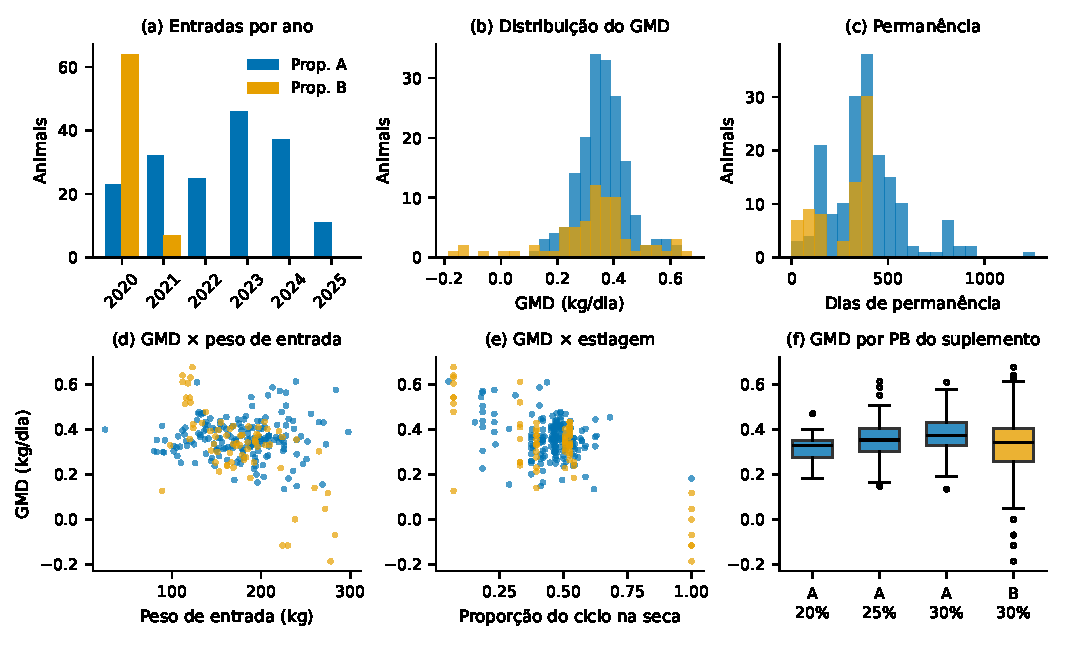
\includegraphics[width=0.88\textwidth]{figs/fig_eda.pdf}
\caption{Panorama do conjunto de 245 animais, por propriedade (A em azul, B em laranja): (a)~entradas por ano; (b)~distribuição do GMD; (c)~dias de permanência; (d)~GMD em função do peso de entrada; (e)~GMD em função da proporção do ciclo na estação seca; (f)~GMD por teor de PB do suplemento.}
\label{fig:eda}
\end{figure*}

Na A, o teor de PB do suplemento tem três níveis (20, 25 e 30\%, com GMD médio de 0,319, 0,352 e 0,379~kg/dia); na B, todos os animais recebem 30\%. A PB da forragem, o número de eventos de transporte e a raça também diferem entre as propriedades: a A tem 10,42\% de PB da forragem, 1 ou 2 eventos de transporte e todos os animais com 75\% de \textit{Bos indicus}; a B tem 10,0\%, 3 eventos e 75\% (37 animais), 100\% (33) ou 50\% (1).

A Figura~\ref{fig:corr} traz a correlação de Pearson de cada variável com o GMD. A mais forte é a proporção do ciclo na seca ($-0{,}61$), mas ela é puxada pelos oito ciclos curtos descritos acima: sem eles, cai para $-0{,}40$. Peso de entrada ($-0{,}25$) e temperatura média ($+0{,}25$) vêm em seguida, e permanência e suplemento médio têm correlação linear próxima de zero ($+0{,}01$ e $+0{,}03$), o que não exclui relações não lineares. Como as variáveis de manejo variam pouco dentro de cada propriedade, elas se confundem com a própria propriedade: PB da forragem e número de eventos de transporte têm correlação de $-0{,}85$ entre si, e temperatura média e proporção de seca, de $-0{,}59$.

\begin{figure}[t]
\centering
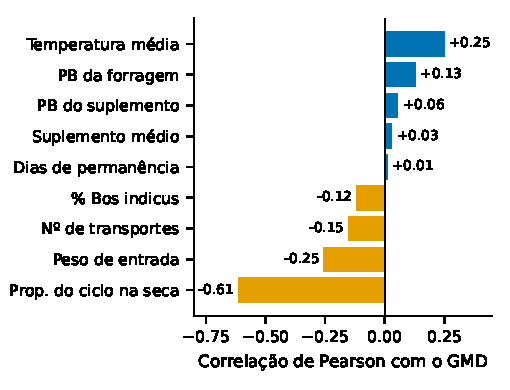
\includegraphics[width=0.95\columnwidth]{figs/fig_corr.pdf}
\caption{Correlação de Pearson entre cada variável preditora e o GMD.}
\label{fig:corr}
\end{figure}

\subsection{Modelos}

\textbf{Regressão linear:} mínimos quadrados ordinários com variáveis padronizadas. \textbf{XGBoost}~\cite{chen2016xgboost}: busca em grade de 48 combinações (200 ou 400 árvores; profundidade 2, 3 ou 4; taxa de aprendizado 0,03 ou 0,1; \textit{subsample} 0,8 ou 1; peso mínimo por folha 1 ou 5); a melhor foi 200 árvores, profundidade 3, taxa 0,1, \textit{subsample} 0,8 e peso mínimo 1.

\textbf{MLP:} rede densa com camadas de 128, 64, 32 e 16 neurônios (12\,641 parâmetros), normalização em lote~\cite{ioffe2015batchnorm} e ReLU após cada camada, saída linear e sem \textit{dropout}. Treino com Adam~\cite{kingma2015adam} (taxa 0,01; decaimento de pesos $10^{-4}$), lotes de 32, perda de Huber~\cite{huber1964robust}, atributos e alvo padronizados (ajuste só no treino), redução da taxa por platô (paciência 40) e parada antecipada (paciência 60) sobre 25\% do treino separados como validação, com no máximo 300 épocas. A arquitetura e os hiperparâmetros vieram de uma grade de 72 configurações (três arquiteturas, \textit{dropout} 0 ou 0,1, três taxas, normalização ligada ou não, decaimento 0 ou $10^{-4}$) e foram então congelados. A MLP reportada é a média das previsões de cinco redes com sementes distintas, implementadas em PyTorch~\cite{pytorch2023}.

\textbf{TabPFN:} modelo de fundação para dados tabulares; a versão descrita por Hollmann et al.~\cite{hollmann2025tabpfn} foi pré-treinada em milhões de conjuntos de dados sintéticos. Não há atualização de pesos: ao receber os animais de treino, o modelo os usa como contexto e prevê os de teste (aprendizado em contexto). Usou-se o \texttt{TabPFNRegressor} padrão do pacote \texttt{tabpfn} 9.0.0 (modelo 3.5~\cite{jager2026tabpfn35}), com atributos não escalonados e sem ajuste de hiperparâmetros.

Um aumento de dados por ruído de medição nos atributos (peso de entrada e temperatura), aplicado só ao treino, foi testado e não trouxe ganho consistente (piorou o XGBoost e o TabPFN, não alterou a regressão linear e elevou o $R^2$ da MLP de 0,843 para 0,861 em uma execução, dentro da variação entre execuções); os resultados reportados não o usam. A regressão linear e as rotinas de validação são do scikit-learn~\cite{pedregosa2011sklearn}.

\subsection{Protocolo de validação}

Três esquemas foram usados, todos com ajuste de escalas apenas no treino.

\textbf{(1)~Validação cruzada por propriedade.} Cinco dobras disjuntas, cada uma com 49 animais de teste estratificados pela propriedade (35 de A e 14 de B em quatro dobras; 34 e 15 na outra), e 196 de treino. Cada animal é testado uma vez.

\textbf{(2)~Treino em uma propriedade, teste na outra.} Treina-se em A e testa-se em B, e vice-versa, sem novo ajuste dos modelos.

\textbf{(3)~Validação cruzada agrupada por lote.} Cinco dobras (\textit{GroupKFold}) em que nenhum lote é dividido entre treino e teste. As dobras têm 49 animais, mas não são estratificadas por propriedade (uma delas contém apenas animais de A). Os modelos usam as configurações já escolhidas, sem novo ajuste.

As métricas são o erro absoluto médio (MAE, em kg/dia) e o coeficiente de determinação $R^2$, calculados em cada dobra e resumidos pela média e pelo desvio-padrão entre dobras. Como referência, usa-se o preditor ingênuo que prevê a média do GMD do treino. A seleção de hiperparâmetros da MLP e do XGBoost usou as mesmas dobras do esquema~(1), o que favorece esses dois modelos nessa comparação; o TabPFN não foi ajustado.

\subsection{Interpretação}

Os valores SHAP~\cite{lundberg2017shap} do TabPFN foram calculados com o \textit{KernelExplainer}, que só exige a função de previsão, com 20 amostras de fundo e número de amostras automático, sobre o modelo ajustado nos 245 animais. Reporta-se o valor absoluto médio por variável.

\section{Resultados}\label{sec:res}

\subsection{Validação cruzada por propriedade}

A Tabela~\ref{tab:cv} mostra o desempenho no esquema (1). O TabPFN obteve o menor erro (MAE de 0,0145~kg/dia, 82\% abaixo do preditor ingênuo, de 0,0796) e o maior $R^2$ (0,863), seguido da MLP (0,820; MAE de 0,0285). O XGBoost e a regressão linear ficaram bem abaixo ($R^2$ de 0,508 e 0,426). O desvio-padrão do $R^2$ entre as dobras é alto, sobretudo para TabPFN, XGBoost e regressão linear: a primeira dobra teve $R^2$ muito menor que as demais para esses três modelos (negativo nos dois últimos, 0,47 no TabPFN).

\begin{table}[t]
\caption{Validação cruzada por propriedade (5 dobras, 49 animais de teste cada). Média $\pm$ desvio-padrão entre dobras. MAE do preditor ingênuo: 0,0796.}
\label{tab:cv}
\centering
\small
\begin{tabular}{@{}lcc@{}}
\toprule
\textbf{Modelo} & \textbf{$R^2$} & \textbf{MAE (kg/dia)} \\
\midrule
TabPFN & $0{,}863 \pm 0{,}220$ & $0{,}0145 \pm 0{,}0072$ \\
MLP (5 sementes) & $0{,}820 \pm 0{,}120$ & $0{,}0285 \pm 0{,}0042$ \\
XGBoost & $0{,}508 \pm 0{,}346$ & $0{,}0512 \pm 0{,}0061$ \\
Regressão linear & $0{,}426 \pm 0{,}352$ & $0{,}0629 \pm 0{,}0063$ \\
\bottomrule
\end{tabular}
\end{table}

\subsection{Validação agrupada por lote}

A Figura~\ref{fig:cv} compara o esquema (1) com a validação agrupada por lote. Todos os modelos pioram quando os lotes não podem ser divididos entre treino e teste: a regressão linear cai de 0,426 para 0,066, o XGBoost de 0,508 para 0,325, o TabPFN de 0,863 para 0,770 e a MLP de 0,841 para 0,760 (o valor de 0,841 vem de uma nova execução das cinco redes; a Tabela~\ref{tab:cv} traz 0,820, e a diferença reflete a variabilidade do treinamento). A ordem entre os modelos se mantém.

\begin{figure}[t]
\centering
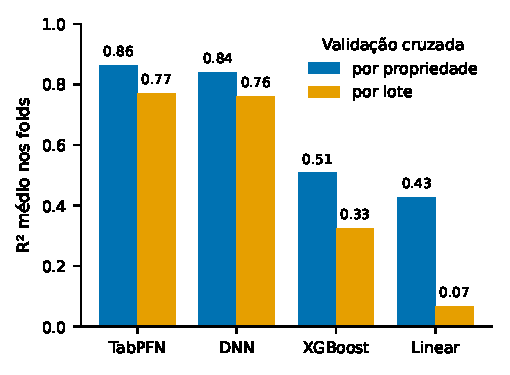
\includegraphics[width=0.95\columnwidth]{figs/fig_esquemas_cv.pdf}
\caption{$R^2$ médio por modelo sob validação cruzada por propriedade e agrupada por lote.}
\label{fig:cv}
\end{figure}

\subsection{Generalização entre propriedades}

A Tabela~\ref{tab:lopo} traz o esquema (2). Ao testar em B, TabPFN, XGBoost e MLP ficaram abaixo do erro do preditor ingênuo (0,1155) e tiveram $R^2$ positivo (0,48, 0,29 e 0,35). Ao testar em A, nenhum modelo superou o preditor ingênuo (0,0704) e os $R^2$ foram muito negativos (de $-0{,}74$ no XGBoost a $-71$ na regressão linear).

\begin{table}[t]
\caption{Treino em uma propriedade e teste na outra. MAE em kg/dia.}
\label{tab:lopo}
\centering
\small
\begin{tabular}{@{}lcccc@{}}
\toprule
 & \multicolumn{2}{c}{\textbf{Teste em A}} & \multicolumn{2}{c}{\textbf{Teste em B}} \\
\cmidrule(lr){2-3}\cmidrule(lr){4-5}
\textbf{Modelo} & $R^2$ & MAE & $R^2$ & MAE \\
\midrule
TabPFN & $-29{,}8$ & 0,242 & 0,48 & 0,072 \\
MLP & $-49{,}3$ & 0,298 & 0,35 & 0,110 \\
XGBoost & $-0{,}74$ & 0,088 & 0,29 & 0,092 \\
Regressão linear & $-71{,}0$ & 0,350 & $-1{,}61$ & 0,249 \\
Ingênuo & -- & 0,070 & -- & 0,116 \\
\bottomrule
\end{tabular}
\end{table}

\subsection{Interpretação}

A Figura~\ref{fig:shap} mostra a importância média dos valores SHAP do TabPFN. Três variáveis concentram 90\% da importância total: peso de entrada (0,171~kg/dia), suplemento médio (0,136) e dias de permanência (0,093). A proporção do ciclo na seca (0,023) é a quarta; temperatura, PB da forragem, transporte, PB do suplemento e proporção \textit{Bos indicus} ficam abaixo de 0,01.

\begin{figure}[t]
\centering
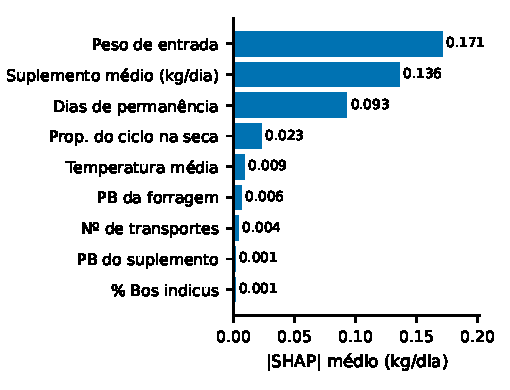
\includegraphics[width=0.95\columnwidth]{figs/fig_shap.pdf}
\caption{Importância média (valor absoluto médio dos SHAP) das variáveis no TabPFN ajustado nos 245 animais.}
\label{fig:shap}
\end{figure}

\section{Discussão}\label{sec:disc}

\textbf{Dentro da distribuição.} TabPFN e MLP lideram a validação por propriedade, à frente do XGBoost e da regressão linear. A diferença entre os dois líderes em $R^2$ (0,863 contra 0,820, ou 0,841 em uma nova execução da MLP) é menor que o desvio entre dobras e que a variação entre execuções da rede, e não é conclusiva; no MAE, a diferença é maior (0,0145 contra 0,0285 kg/dia), mas com cinco dobras não há como atribuir significância estatística. A seleção de hiperparâmetros nas mesmas dobras da avaliação favorece a MLP e o XGBoost; o TabPFN, usado sem ajuste, não se beneficia disso, de modo que sua vantagem não decorre desse viés.

\textbf{Validação por lote.} Os animais de um lote compartilham a janela de datas e, portanto, valores quase idênticos de temperatura e proporção de seca. Retirar lotes inteiros do treino reduziu o $R^2$ de todos os modelos, o que mostra que parte do desempenho na validação por propriedade depende de lotes semelhantes aos vistos no treino. A queda foi maior para a regressão linear ($-0{,}36$) e menor para TabPFN e MLP ($-0{,}09$ e $-0{,}08$).

\textbf{Entre propriedades.} Nenhum resultado indica generalização confiável. Ao testar em A, o desempenho piora para todos os modelos e nenhum supera o preditor ingênuo. Treinar com os 71 animais de B (7 lotes e um único teor de PB do suplemento) para prever os 174 de A (59 lotes e três teores) é um problema de extrapolação: a regressão linear e o TabPFN extrapolam mal fora da faixa de treino, e o XGBoost, por ser constante fora dela, satura, o que é consistente com ele ter o menor erro nessa direção. Ao testar em B, os $R^2$ positivos de TabPFN, MLP e XGBoost sugerem alguma transferência, mas B tem apenas 7 lotes e a estimativa é instável.

\textbf{Leitura do SHAP.} Peso de entrada, suplemento médio e permanência são as variáveis em que o TabPFN mais se apoia. A importância SHAP descreve o comportamento do modelo, não relações causais. A baixa importância de temperatura, PB da forragem, transporte e raça também não indica ausência de efeito: a PB da forragem tem apenas dois valores (um por propriedade) e correlaciona-se fortemente com o número de eventos de transporte ($r=-0{,}85$), o que impede separar seus efeitos neste conjunto.

\textbf{Limitações.} O conjunto é pequeno (245 animais), de apenas duas propriedades e só de fêmeas. O GMD vem de duas pesagens, e os valores negativos ocorrem em ciclos de 43 dias, nos quais o erro de pesagem pesa mais. Não há dados sanitários nem genéticos. Cinco dobras geram estimativas com grande desvio e sem testes de significância. A seleção de hiperparâmetros não foi aninhada na validação, a MLP varia entre execuções, a validação por lote não é estratificada por propriedade, e o TabPFN foi usado em uma única versão.

\section{Conclusão}\label{sec:concl}

Comparamos regressão linear, XGBoost, uma MLP e o TabPFN na estimativa do GMD de 245 bovinos de duas propriedades. Com a validação cruzada por propriedade, TabPFN e MLP superaram os demais ($R^2$ de 0,86 e 0,82; MAE de 0,015 e 0,028~kg/dia). A validação agrupada por lote reduziu o $R^2$ de todos os modelos, mais ainda o da regressão linear, e nenhum modelo generalizou de forma confiável para a outra propriedade.

Como trabalhos futuros, propõem-se: adotar validação aninhada e mais dobras; ampliar o número de propriedades, de lotes e de ciclos; incorporar variáveis sanitárias e genéticas; e explorar a incerteza das previsões, que o TabPFN permite estimar.

\bibliographystyle{IEEEtran}
\bibliography{referencias}

\end{document}
